\section{Entanglement and Operator Spreading in Quantum Circuits} \label{sec:circuits}

\subsection{Circuit Architectures} \label{sub:arch}

Instead of evolving the spin chains with Hamiltonians, we can focus on quantum circuits. Like the earlier systems, circuits consist of chains of Hilbert spaces. Instead of evolving under a time-independent hamiltonian, they evolve with unitary operators, called gates, at discrete times. Simple circuits only contain 2-site gates which act on the product of Hilbert spaces at adjacent sites. 

We could study the dynamics of a single circuit, in analogy with the single hamiltonian studied in the previous section. However, it is also instructive to look at ensembles of circuits, with some type of randomness. This section presents two sources of randomness, the choice of gates and their locations in the circuit.

%References~\cite{Keyserlingk} and~\cite{Nahum2017} both discuss circuits of this type. Both discuss random circuits, although with different sources of randomness. 
One source is the unitary operator chosen at each site at each time. Different gates result in different architectures. 
If the Hilbert space at each site is $q$ dimensional, the space of 2-site unitary matrices is $q^2\times q^2$ dimensional. To find representative behavior, each circuit is made by drawing gates from some distribution. The circuits can then be averaged over these choices. 

Another source of randomness is the placement of the gates. The ``brickwork" model~\cite{Keyserlingk} uses a deterministic architecture, in which at odd times there is a gate to the right of every odd site, while for even times there is a gate to the right of every even site. The ``random" architecture~\cite{Nahum2017} chooses a random site for a single gate at each time step $t = n/\Gamma$, where $\Gamma$ is the gate rate and $n$ is an integer. The placement is then averaged over. The random architecture is equivalent to placing gates at each site in continuous time with Poisson-distributed time steps~\cite{Nahum2017}.

We will first discuss the brickwork circuit, shown in figure~\ref{fig:brickcircuit}.\footnotetext{Redo this figure without course graining, or with new labels.}
\begin{figure}
	\centering
	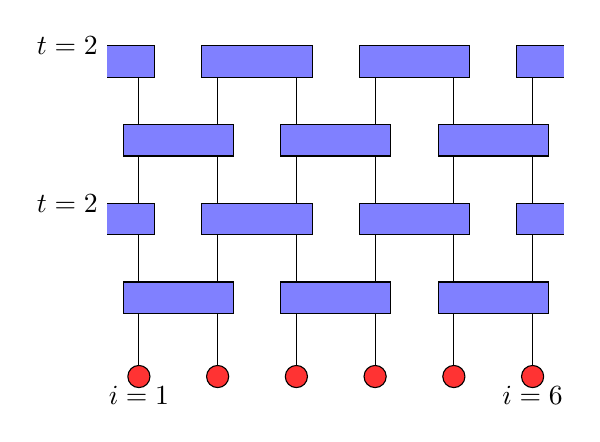
\begin{tikzpicture}[scale = 1]
\draw (0,0) node[below]{$i=1$} -- (0,4);
\filldraw[color=black, fill=red!80] (0,0) circle (4pt) node[anchor=west] { };
\draw (1,0) -- (1,4);
\filldraw[color=black, fill=red!80] (1,0) circle (4pt) node[anchor=west] { };
\draw (2,0) -- (2,4);
\filldraw[color=black, fill=red!80] (2,0) circle (4pt) node[anchor=west] { };
\draw (3,0) -- (3,4);
\filldraw[color=black, fill=red!80] (3,0) circle (4pt) node[anchor=west] { };
\draw (4,0) -- (4,4);
\filldraw[color=black, fill=red!80] (4,0) circle (4pt) node[anchor=west] { };
\draw (5,0) node[below]{$i=6$} -- (5,4);
\filldraw[color=black, fill=red!80] (5,0) circle (4pt) node[anchor=west] { };

\foreach \x/\y in {0/1, 2/1, 4/1, 1/2, 3/2, 0/3, 2/3, 4/3, 1/4, 3/4} 
\filldraw[color=black, fill=blue!50] (\x-.2,\y-.2) rectangle (\x+1.2,\y+.2);

\draw[fill=blue!50] (-.4,1.8) -- (.2,1.8) -- (.2,2.2) -- (-.4,2.2)
								node[left] {$t=2$};
\draw[fill=blue!50] (-.4,3.8) -- (.2,3.8) -- (.2,4.2) -- (-.4,4.2)
								node[left] {$t=2$};
\draw[fill=blue!50] (5.4,4.2) -- (4.8,4.2) -- (4.8,3.8) -- (5.4,3.8);
\draw[fill=blue!50] (5.4,2.2) -- (4.8,2.2) -- (4.8,1.8) -- (5.4,1.8);

%\draw (2.5,4.5) node{$x$};
%\draw[dashed] (2.5,4.2) .. controls (2.5,3.5) .. (3,3.5) 
%                        .. controls (3.5,3.5) .. (3.5,3) 
%                        .. controls (3.5,2.5) .. (3,2.5) 
%                        .. controls (2.5,2.5) .. (2.5,2) 
%                        .. controls (2.5,1.5) .. (3,1.5) 
%                        .. controls (3.5,1.5) .. (3.5,1) 
%                        .. controls (3.5,0.5) .. (3.5,0.5) 
%                        .. controls (3.5,0.0) .. (3.5,0);
\end{tikzpicture}
	\caption{\textbf{Brickwork circuit architecture}. The red circles represent the initial states of the system, while the blue rectangles are unitary gates that evolve the system in time. The Hilbert space at each site is $q$-dimensional, meaning the gates are $q^2\times q^2$ matrices, chosen from the Haar distribution. Taken from~\cite{Keyserlingk}.}
	\label{fig:brickcircuit}
\end{figure}
In this model, each gate is chosen from the Haar distribution, which is invariant to rotations in the space of 2-site operators. Since these act on a $q^2$-dimensional Hilbert space, there are $q^4$ independent operators, including one trivial operator (the identity). 

We want to know how the Pauli end-weight $W(t,i)$ evolves in time in these circuits. Recall that, given an observable $\cal{O}(t)$ evolving in time, this measure how far $\cal{O}$ has spread. Consider the components of the operator that are identities after site $i$, which will have weight $W(t, i)$ by definition. Of the $q^2$ operators that can act on sites $i$ and $i+1$, $q^2$ will be trivial on the second site. Since these will not advance the Pauli end-weight, they do not contribute to operator spreading. 

\emph{Show an explicit example of this for $q=2$}

If some component of the observable ends on site $i+1$, the unitary can move the end back, if it evolves the observable at $i+1$ to the identity. Again, $q^2$ of the 2-site operators contain this specific unitary acting on the second site, so that the probability of moving weight from site $i+1$ to $i$ is the same as not moving the weight from $i$ to $i+1$.

Since the identity will never contribute to operator spreading, we can exclude it from our set of gates. Then, $q^4-q^2$ operators move the Pauli weight. The probability that a random gate advances $W(t,i)$ is $p = \frac{q^2}{q^2+1}$, so that $1-p = \frac{1}{q^2+1}$. After averaging over the possible circuits, this leads to the dynamics of $W(t,i)$, from~\cite{Keyserlingk}
\begin{align}
W(t+1, i) = (1-p)\left(W(t, i) + W(t, i+1)\right)\nn
W(t+1, i+1), = p\left(W(t, i) + W(t, i+1)\right).
\end{align}

[\emph{How much more detail should I go into before this just becomes a synopsis of their paper?}]

The butterfly speed is
\begin{align}
v_B= \frac{q^2-1}{q^2+1}. \label{eqn:keysvb}
\end{align}
The entanglement speed is 
\begin{align}
v_E = \frac{\log\frac{q+q^{-1}}{2}}{\log q} = \frac{\log\left(1-v_B^2
	\right)}{\log\left(\frac{1-v_b}{1+v_B}\right)}.\label{eqn:keysve}
\end{align}
These speeds describe operator spreading represented in figure~\ref{fig:onesite_spreading}.
\begin{figure}
	\centering
	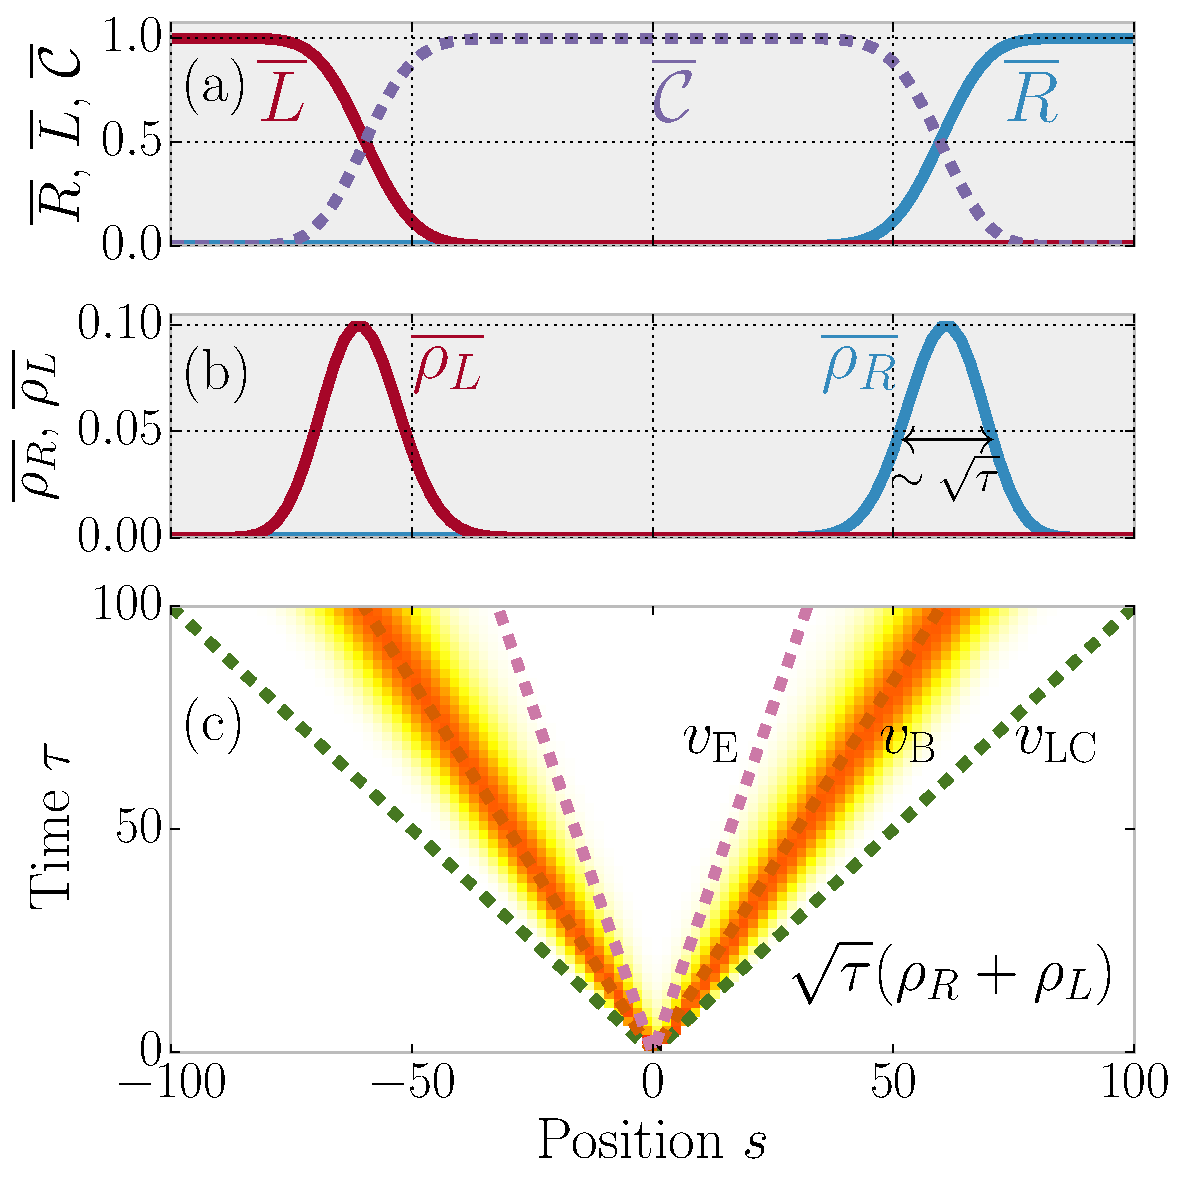
\includegraphics[width=.5\linewidth]{onesite_spreading}
	\caption{\textbf{Operator spreading in a brickwork circuit}. $\bar{\rho_R}$ is what is here called $W(t,i)$. From~\cite{Keyserlingk}.}
	\label{fig:onesite_spreading}
\end{figure}
An initially local operator spreads with velocity $v_B$, and diffuses at a rate related to $v_E$. 

\subsection{Deterministic Limit}  \label{sub:determ}

Take the large $q$ limit of equations~\ref{eqn:keysvb} and~\ref{eqn:keysve}
\begin{align}
v_B &\simeq 1-\frac{2}{q^2},\nn
v_E &\simeq 1-\frac{\log 2}{\log q}.
\end{align}
Since both speeds approach the light cone velocity (defined to be 1), an initial perturbation does not spread in time, and travels at the light cone velocity. In figure~\ref{fig:onesite_spreading}, this would be represented by $\bar{R}$ and $\bar{L}$ becoming step functions and $W(t,i)$ becoming a delta function.

\emph{What are the two velocities in the random circuit architecture now?}

\emph{Make the connection to bipartite entanglement entropy for a state}

We know then that, except for fine-tuned operators that are measure zero on the Haar distribution, the random two-site gate will maximize bipartite entanglement entropy. From equation~\ref{eqn:offbyone} the maximum entanglement possible across cut $x$ is 
\begin{align}
S(x) \le \min\left\lbrace S(x-1), S(x+1)\right\rbrace + 1. \nonumber
\end{align}
Furthermore, a gate acting across cut $x$ does not affect $S(x-1)$ or $S(x+1)$.

Taken together, these facts mean that after a gate across cut $x$, the new entanglement entropy is~\cite{Buyskikh2016}~\emph{Make sure this is actually in this source}
\begin{align}
S(x, t+1) = \min\left\lbrace S(x-1, t), S(x+1, t)\right\rbrace + 1.
	\label{eqn:update}
\end{align}
Then if at any point $S(x)$ becomes integer valued, it remains so for the rest of the evolution. There are a few pictures that make this integer-valued evolution more intuitive.

\subsubsection{Surface Growth Picture}  \label{subsub:surfgrowth}

One model for the entropy growth described above is the Tetris-like surface growth picture. Here, the entropy is represented by a piecewise-constant function with the height given by the entropy across each cut, as in figure~\ref{fig:tetris}, taken from \cite{Nahum2017}. 
\begin{figure}
	\centering
	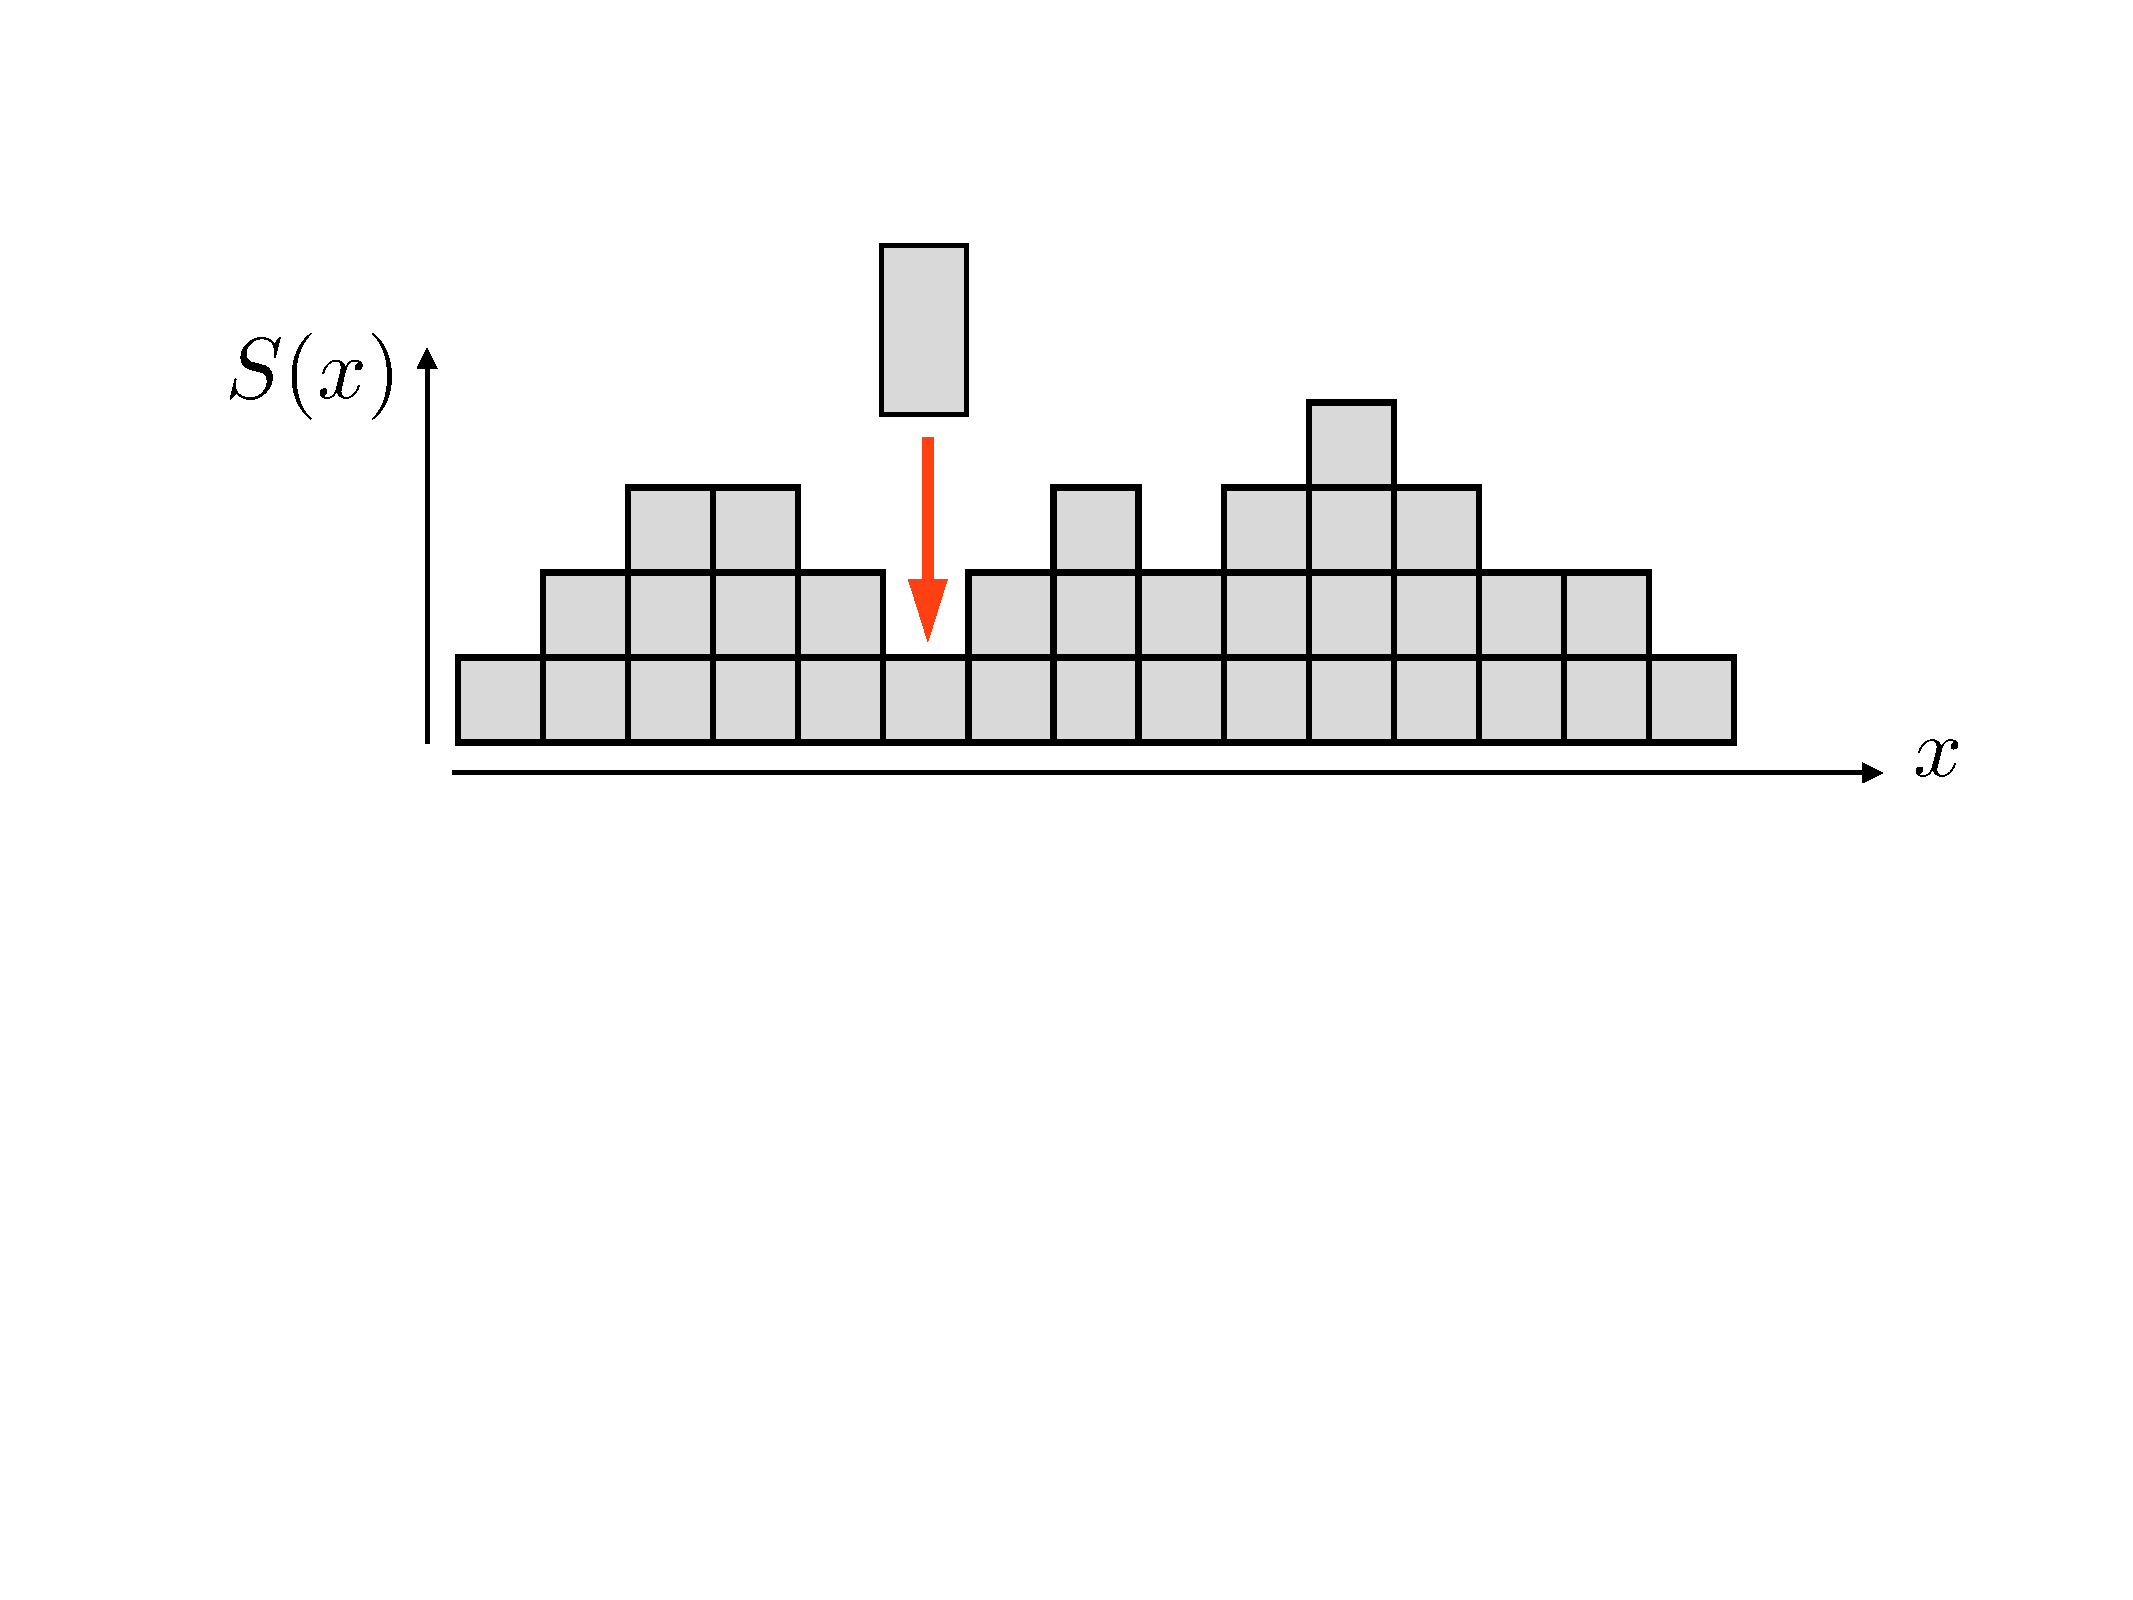
\includegraphics[width=.5\textwidth]{tetris.pdf}
	\caption{\textbf{Tetris-like model for large-$q$ chain.} The gate at cut $x$ adds enough entropy so that $S(x)$ is one greater than either of its neighbors. Figure from~\cite{Nahum2017}.}
	\label{fig:tetris}
\end{figure}
In general, it is possible for the entropy across two adjacent cuts to be equal. However, figure~\ref{fig:applyingUnitary}, also from~\cite{Nahum2017}, shows that flat sections can be destroyed but not created. 
\begin{figure}
	\centering
	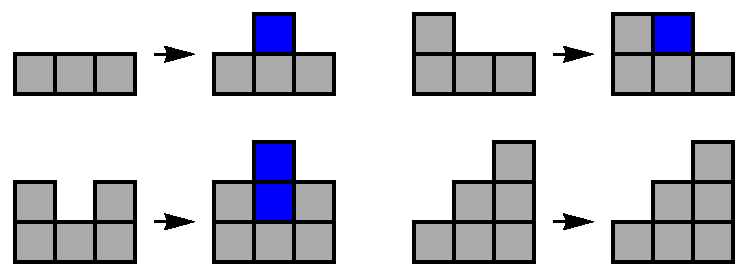
\includegraphics[width=.5\textwidth]{applyingUnitary.pdf}
	\caption{\textbf{Several possibilities for local changes} in the large $q$ model. If three adjacent cuts all have equal entropy, the two flat sections annihilate each other. There is no way to generate flat sections.}
	\label{fig:applyingUnitary}
\end{figure}

It makes sense then to only consider states that have no flat sections, so that $S(x) = S(x-1)\pm1$ for all $x$. In this case, instead of a picture like figure~\ref{fig:tetris} it is possible to represent the entropy at each bond as a point, with a diagonal slope connecting bonds. The slope between cuts (at a site) will always be $\pm1$. Instead of $2\times1$ or $1\times1$ rectangles, the gates are then squares coming down point-first, as in figure~\ref{fig:diaggate}. 
\begin{figure}
	\centering
	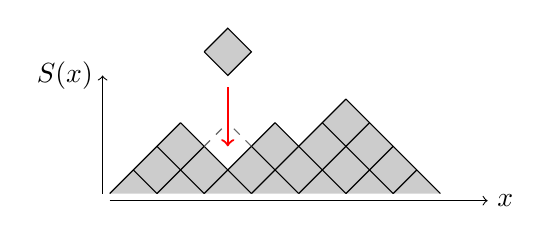
\begin{tikzpicture}[scale = .3]
\draw[->] (0, -.3) -- (16,-.3) node[right]{$x$};
\draw[->] (-.3,0) -- (-.3,5) node[left]{$S(x)$};
\fill[black!20] (0,0) -- (3,3) -- (5,1) -- (7,3) -- (8,2) --
				(10,4) -- (14,0) ;
\draw (0,0) -- (3,3);
\draw (2,0) -- (4,2);
\draw (4,0) -- (7,3);
\draw (6,0) -- (10,4);
\draw (8,0) -- (11,3);
\draw (10,0) -- (12,2);
\draw (12,0) -- (13,1);
\draw (2,0) -- (1,1);
\draw (4,0) -- (2,2);
\draw (6,0) -- (3,3);
\draw (8,0) -- (6,2);
\draw (10,0) -- (7,3);
\draw (12,0) -- (9,3);
\draw (14,0) -- (10,4);
\draw[dashed, black!60]  (4,2) -- (5,3);
\draw[dashed, black!60]  (6,2) -- (5,3);

\draw[fill=black!20] (4,6) -- (5,5) -- (6,6) -- (5,7) -- (4,6);
\draw[thick, ->, red] (5,4.5) -- (5,2);
\end{tikzpicture}
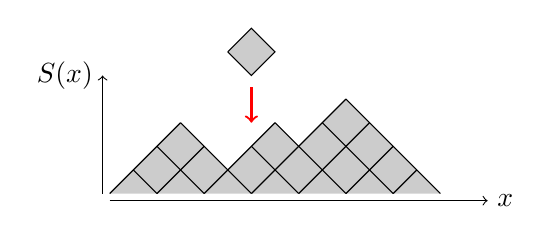
\begin{tikzpicture}[scale = .3, cross/.style={path picture={ 
		\draw[black]
		(path picture bounding box.south east) -- (path picture bounding box.north west) (path picture bounding box.south west) -- (path picture bounding box.north east);
}}]

\draw[->] (0, -.3) -- (16,-.3) node[right]{$x$};
\draw[->] (-.3,0) -- (-.3,5) node[left]{$S(x)$};
\fill[black!20] (0,0) -- (3,3) -- (5,1) -- (7,3) -- (8,2) --
(10,4) -- (14,0) ;
\draw (0,0) -- (3,3);
\draw (2,0) -- (4,2);
\draw (4,0) -- (7,3);
\draw (6,0) -- (10,4);
\draw (8,0) -- (11,3);
\draw (10,0) -- (12,2);
\draw (12,0) -- (13,1);
\draw (2,0) -- (1,1);
\draw (4,0) -- (2,2);
\draw (6,0) -- (3,3);
\draw (8,0) -- (6,2);
\draw (10,0) -- (7,3);
\draw (12,0) -- (9,3);
\draw (14,0) -- (10,4);
%\draw[dashed, black!60]  (5,3) -- (6,4);
%\draw[dashed, black!60]  (7,3) -- (6,4);
%\draw[dashed, black!60]  (6,2) -- (5,3);

\draw[fill=black!20] (5,6) -- (6,5) -- (7,6) -- (6,7) -- (5,6);
\draw[thick, ->, red] (6,4.5) -- (6,3);
%\node [draw,circle,cross,minimum width=1](B) at (6,3.5){}; 
\end{tikzpicture}

	\caption{\textbf{Another picture of the configuration in figure~\ref{fig:tetris}}. Here the cut positions are top or bottom vertices of the squares. On the left, the gate at time $t$ results in entropy growth at $x$ because at time $t-1$, $S(x-1) > S(x) < S(x+1)$. On the right the gate has no effect. Although $S(x) < S(x+1)$, the case $S(x) < S(x-1)$ is not satisfied. }
	\label{fig:diaggate}
\end{figure}
If the gate falls on a local minimum, it lifts the entropy at that bond. If the gate falls on a local maximum or a non-extremum it has no effect.

\subsubsection{Minimal Cut Picture} \label{subsub:mincut}

Using the fact that a productive gate raises the entropy at a cut by 2, we can use another picture of the dynamics based on figure~\ref{fig:brickcircuit}. Assume the initial state is a product state so the entropy at each cut is initially 0 and evolve with a brickwork circuit. Then after one of the first gates (for example between $i=3$ and $i=4$) the entropy at that cut will become 1. After any of the subsequent gates the entropy at the affected cut increases by 2.

The minimal cut picture~\cite{Nahum2017}\footnote{This might not be the original source} reproduces this behavior by considering cuts through the circuit, as in figure~\ref{fig:mincut}.
\begin{figure}
	\centering
	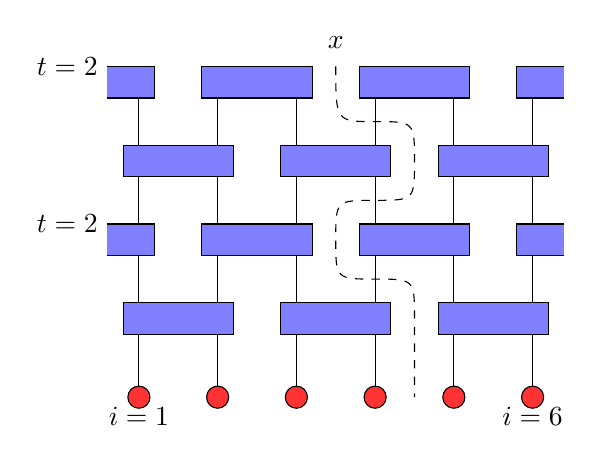
\begin{tikzpicture}[scale = 1]
\draw (0,0) node[below]{$i=1$} -- (0,4);
\filldraw[color=black, fill=red!80] (0,0) circle (4pt) node[anchor=west] { };
\draw (1,0) -- (1,4);
\filldraw[color=black, fill=red!80] (1,0) circle (4pt) node[anchor=west] { };
\draw (2,0) -- (2,4);
\filldraw[color=black, fill=red!80] (2,0) circle (4pt) node[anchor=west] { };
\draw (3,0) -- (3,4);
\filldraw[color=black, fill=red!80] (3,0) circle (4pt) node[anchor=west] { };
\draw (4,0) -- (4,4);
\filldraw[color=black, fill=red!80] (4,0) circle (4pt) node[anchor=west] { };
\draw (5,0) node[below]{$i=6$} -- (5,4);
\filldraw[color=black, fill=red!80] (5,0) circle (4pt) node[anchor=west] { };

\foreach \x/\y in {0/1, 2/1, 4/1, 1/2, 3/2, 0/3, 2/3, 4/3, 1/4, 3/4} 
\filldraw[color=black, fill=blue!50] (\x-.2,\y-.2) rectangle (\x+1.2,\y+.2);

\draw[fill=blue!50] (-.4,1.8) -- (.2,1.8) -- (.2,2.2) -- (-.4,2.2)
								node[left] {$t=2$};
\draw[fill=blue!50] (-.4,3.8) -- (.2,3.8) -- (.2,4.2) -- (-.4,4.2)
								node[left] {$t=2$};
\draw[fill=blue!50] (5.4,4.2) -- (4.8,4.2) -- (4.8,3.8) -- (5.4,3.8);
\draw[fill=blue!50] (5.4,2.2) -- (4.8,2.2) -- (4.8,1.8) -- (5.4,1.8);

\draw (2.5,4.5) node{$x$};
\draw[dashed] (2.5,4.2) .. controls (2.5,3.5) .. (3,3.5) 
                        .. controls (3.5,3.5) .. (3.5,3) 
                        .. controls (3.5,2.5) .. (3,2.5) 
                        .. controls (2.5,2.5) .. (2.5,2) 
                        .. controls (2.5,1.5) .. (3,1.5) 
                        .. controls (3.5,1.5) .. (3.5,1) 
                        .. controls (3.5,0.5) .. (3.5,0.5) 
                        .. controls (3.5,0.0) .. (3.5,0);
\end{tikzpicture}
	\caption{\textbf{Minimal cut picture.} Assuming an initial product state, $S(y)$ is given by the minimal number of legs that must be cut to draw a line from the bottom of the circuit to $y$. Cutting through gates is not allowed (or equivalently costs two cuts) and the initial point need not be $y$. Figure adapted from~\cite{Nahum2017}.}
	\label{fig:mincut}
\end{figure}
To find the entanglement across $y$, start in an unentangled state. If the initial state is entangled, include gates for $t<0$ that evolve a product state into the initial state at time $t=0$. Then, starting at the top of the circuit at $y$, find the path through the circuit that cuts through no gates and through the fewest of the lines defined by sites, called legs. The path need not end at $y$. The entanglement at $y$ is the number of legs cut by this path. 

For the brickwork circuit, this reproduces the entropy calculation quoted above, with first gates generating 1 unit of entanglement and subsequent gates generating 2. However, in circuits where not every gate is productive, the min-cut picture still works, and agrees with the surface growth picture.

Consider the circuit in figure~\ref{fig:degeneratemincut}.
\begin{figure}
	\centering
	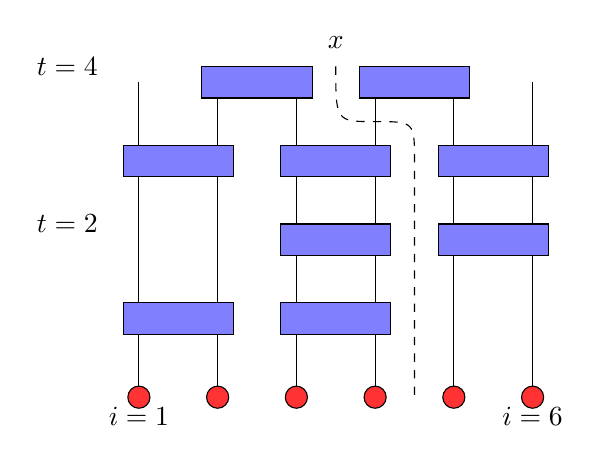
\begin{tikzpicture}[scale = 1]
\draw (0,0) node[below]{$i=1$} -- (0,4);
\filldraw[color=black, fill=red!80] (0,0) circle (4pt) node[anchor=west] { };
\draw (1,0) -- (1,4);
\filldraw[color=black, fill=red!80] (1,0) circle (4pt) node[anchor=west] { };
\draw (2,0) -- (2,4);
\filldraw[color=black, fill=red!80] (2,0) circle (4pt) node[anchor=west] { };
\draw (3,0) -- (3,4);
\filldraw[color=black, fill=red!80] (3,0) circle (4pt) node[anchor=west] { };
\draw (4,0) -- (4,4);
\filldraw[color=black, fill=red!80] (4,0) circle (4pt) node[anchor=west] { };
\draw (5,0) node[below]{$i=6$} -- (5,4);
\filldraw[color=black, fill=red!80] (5,0) circle (4pt) node[anchor=west] { };

\foreach \x/\y in {0/1, 0/3, 2/1, 2/2, 2/3, 4/2, 4/3, 1/4, 3/4} 
\filldraw[color=black, fill=blue!50] (\x-.2,\y-.2) rectangle (\x+1.2,\y+.2);

\draw[fill=blue!50] (-.4,2.2) node[left] {$t=2$};
\draw[fill=blue!50] (-.4,4.2) node[left] {$t=4$};

\draw (2.5,4.5) node{$x$};
\draw [dashed] (2.5,4.2) .. controls (2.5,3.5) .. (3,3.5) 
                         .. controls (3.5,3.5) .. (3.5,3) 
                         .. controls (3.5,1.5) .. (3.5,1) 
                         .. controls (3.5,0.5) .. (3.5,0.5) 
                         .. controls (3.5,0.0) .. (3.5,0);
\end{tikzpicture}
	\caption{\textbf{Minimal cut with degenerate gates.} All gates at cut $y$ after the first gate there produce no entanglement because $S(y)$ is a local maximum.}
	\label{fig:degeneratemincut}
\end{figure}
After the initial gate acts between sites 3 and 4, $S(y)$ becomes a local maximum, with so that all gates after it become unproductive. In the surface growth picture this is represented by multiple gates falling on a local maximum. This is to show that the min-cut picture agrees with the surface growth picture, and provides another set of intuition for the dynamics of this class of circuits.

\emph{Entanglement from (x,0) to (y,t)}

\subsection{Coarse Graining and Long Wavelength Dynamics} \label{sub:coarse}

It is possible to abstract out even more of the detailed dynamics to consider the large scale behavior. To do this, interpret $S(x)$ as a continuous real valued function. The entanglement growth rate can be calculated under the assumption that up and down steps (from the picture in figure~\ref{fig:diaggate}) are uncorrelated and the large scale slope $\pd{S}{x}$ is constant. 

For an entropy surface with constant slope $m\equiv\pd{S}{x}$ and no correlations, each step from one site to the next has probability $\frac{1+m}{2}$ of being up and $\frac{1-m}{2}$ of being down. The assumption that there are no correlations is exact in the random architecture. Consider a gate operating on cut $x$ at time $t$. For the gate to increase the entropy $S(x)$, it must be the case that $S(x)<S(x-1), S(x+1)$. The probability of this is $\frac{1+m}{2} \frac{1-m}{2} = \frac{1-m^2}{4}$. In this case we have $S(x,t+1)=S(x,t)+2$, because the gate increases the entropy to be great than that of its neighbors. Then if the gates arrive with a rate $\Gamma$, the entanglement growth rate is
\begin{align}
\pd{S}{t} = \Gamma\frac{1-m^2}{2}\equiv G(m).
\end{align}
Useful checks of this formula are that the entropy does not increase at maximal or minimal slope $m=1,-1$, and that at $m=0$, $\pd{S}{t}=\Gamma/2$, 1/4 the brickwork value. The latter rate makes sense because in the case of the brickwork circuit all gates are guaranteed to raise the entropy, while here only 1/4 will have an effect.

At the maximal values of $m=\pm1$, the dependence of $G$ on $m$ is 
\begin{align}
\left.\pd{G}{m}\middle|_{m=\pm 1}=\Gamma\frac{-2m}{2}\right|_{m=\pm 1} = \mp \Gamma,
\end{align}
the entanglement velocity calculated in~\ref{sub:determ}. This correspondence between the extremal slope of the entanglement growth rate and the entanglement velocity\footnote{$v_E$ or $v_B$?} described in section~\ref{sec:opsp}. The surface growth picture provides a new description of this connection.

When the slope is near its largest possible value, so that the entropy increases at nearly every site, it is possible to isolate the behavior of the few down steps. Figure~\ref{fig:particle} shows such a configuration.
\begin{figure}
	\centering
	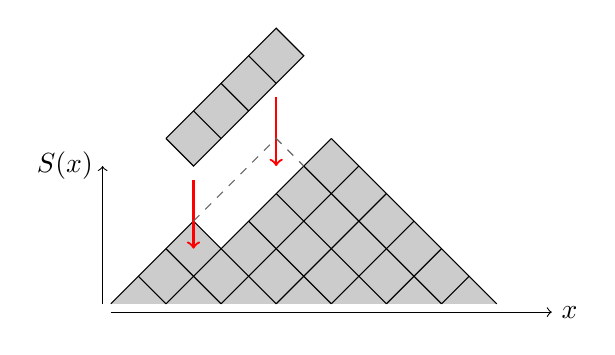
\begin{tikzpicture}[scale = .35]
\draw[->] (0, -.3) -- (16,-.3) node[right]{$x$};
\draw[->] (-.3,0) -- (-.3,5) node[left]{$S(x)$};
\fill[black!20] (0,0) -- (3,3) -- (4,2) -- (8,6) -- (14,0) ;
\draw (0,0) -- (3,3);
\draw (2,0) -- (8,6);
\draw (4,0) -- (9,5);
\draw (6,0) -- (10,4);
\draw (8,0) -- (11,3);
\draw (10,0) -- (12,2);
\draw (12,0) -- (13,1);
\draw (2,0) -- (1,1);
\draw (4,0) -- (2,2);
\draw (6,0) -- (3,3);
\draw (8,0) -- (5,3);
\draw (10,0) -- (6,4);
\draw (12,0) -- (7,5);
\draw (14,0) -- (8,6);

\draw[fill=black!20] (2,6) -- (3,5) -- (4,6) -- (5,7) -- (6,8) -- (7,9) --
					 (6,10) -- (3,7) -- (2,6);
\draw (4,6) -- (3,7);
\draw (5,7) -- (4,8);
\draw (6,8) -- (5,9);
%\draw (9,9) -- ()
\draw[thick, ->, red] (3,4.5) -- (3,2);
\draw[thick, ->, red] (6,7.5) -- (6,5);

\draw[dashed, black!60] (3,3) -- (6,6) -- (7,5);
\end{tikzpicture}
	\caption{\textbf{Near-maximal slope}. The single down step acts like a particle in the system. The 4 consecutive gates have the effect of moving the particle 3 sites to the right.}
	\label{fig:particle}
\end{figure}
Since gates can only act between a down step and an up step, these ``particles"\footnote{Define the particle as existing at site or cut?} follow a deterministic behavior and control the entropy growth in the circuit. 

Consider a series of consecutive gates with its first gate acting between sites $i$ and $i+1$ and its last gate between $j$ and $j+1$. Series of gates like this (called staircases) are discussed in section~\ref{sec:stairs}. If there are no down steps in this region, the gate has no effect. If there is a single down step between sites $i$ and $j$, inclusive, that step gets moved to site $j+1$. More down steps will interact with each other but at the present we are only considering configurations with isolated down steps. 

Now consider an operator with the last non-identity contribution at a site between $i$ and $j$, inclusive. With probability 1, the series of gates in the last paragraph move the end of the operator to site $j+1$. This should demonstrate that operator ends and down step ``particles" have the same dynamics. 

The speed of the end of the operator is $v_B$. It is not immediately clear how the speed of the particle, call it $v_p$, should be related. If, in time $t$ the particle moves $v_pt$ sites, it has increased the \dots

\emph{Finish this description. Does it really belong here though? If so, make sure to show that particles don't approach each other, but do repel each other if they're too close.}